\documentclass{article}
 
\usepackage{arxiv}
 
\usepackage[utf8]{inputenc} % allow utf-8 input
\usepackage[T1]{fontenc}    % use 8-bit T1 fonts
\usepackage{hyperref}       % hyperlinks
\usepackage{url}            % simple URL typesetting
\usepackage{booktabs}       % professional-quality tables
\usepackage{amsfonts}       % blackboard math symbols
\usepackage{nicefrac}       % compact symbols for 1/2, etc.
\usepackage{microtype}      % microtypography
\usepackage{listings} % displaying code
\usepackage{lipsum}   % Can be removed after putting your text content
\usepackage{graphicx}
\usepackage{tabto}
 
\title{Is It Normal: A Novel Approach of Utilizing Python 3.6 to Generate a Normal Gaussian Distribution}
 
%\date{September 9, 1985} % Here you can change the date presented in the paper title
%\date{}          % Or removing it
 
\lstset
{ %Formatting for code in appendix
    language=Python,
    basicstyle=\footnotesize,
    numbers=left,
    stepnumber=1,
    showstringspaces=false,
    tabsize=1,
    breaklines=true,
    breakatwhitespace=false,
}
 
\author{
  Deepak ~Ramalingam \\
  High School Senior \\
  Monta Vista High School\\
  Cupertino, California 95014 \\
  \texttt{rdeepak2002@gmail.com} \\
   \And
 Kirtan U.~Shah \\
  High School Senior\\
  Monta Vista High School\\
  Cupertino, California 95014 \\
  \texttt{kirtan.u.shah@gmail.com} \\
}
 
% Uncomment to override  the `A preprint' in the header
\renewcommand{\headeright}{}
 
\begin{document}
\maketitle
 
\begin{abstract}
The following paper describes the manner in which we generated a normal gaussian distribution by utilizing the Python 3.6 programming language in order to create a program, program.py, to read in a text file containing the first one million digits of pi and output the average of every 5 digits to a new text file, then using the Google Sheets web application in order to create a visual histogram using the outputted data.
\end{abstract}
 
\section{Histogram}
 
\centerline{\textbf{Figure 1}}
 
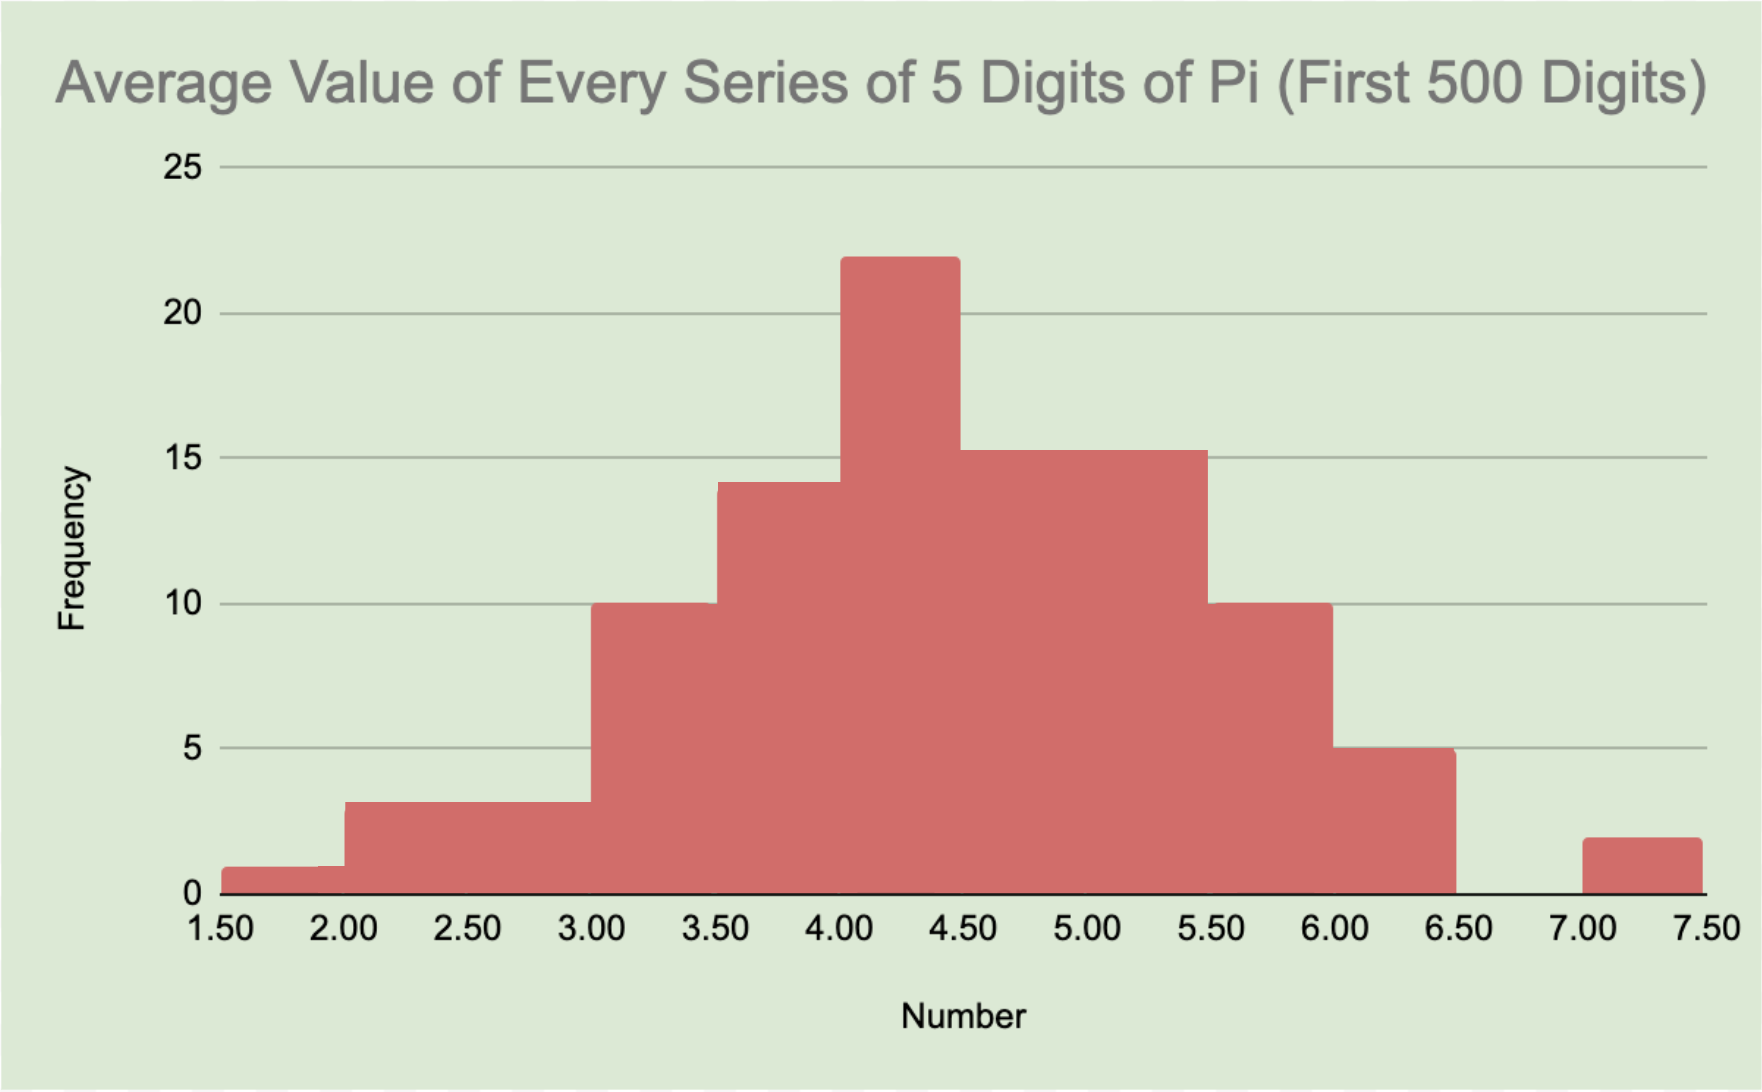
\includegraphics[width=\textwidth]{histogram.png}
 
\section{Introduction}
We received the first one million digits of pi as a text file from https://www.angio.net/pi/digits.html, then we used the Python 3.6 programming language to create the code seen in figure 2. This code reads the first million digits of pi as from the text file, then uses a for loop in order to average every 5 digits of pi. We chose this as our data because we are interested in relating statistics to the irrational number pi, which is used in wave functions and calculating circular properties.
 
\vspace{20px}
 
\centerline{\textbf{Figure 2}}
 
\begin{lstlisting}
limit = 60000
avgNum = 5
 
f = open("pimil.txt")
 
pi = f.read()
pi = pi.replace("\n", "")
pi = pi.replace(" ", "")
 
f2 = open("output.txt", "r+")
 
avg = 0.0
 
for i in range(0, limit, avgNum):
  substr = pi[i:i+avgNum]
  for j in range(avgNum):
    avg += int(substr[j])
  avg = avg / avgNum
  f2.write(str(avg) + "\n")
  avg = 0.0
\end{lstlisting}
 
\section{Description}
\begin{center}
  \begin{tabular}{||c | c | c | c | c | c | c||}
  \hline\hline
  Minimum & First Quartile & Median & Third Quartile & Maximum & Mean & Standard Deviation\\ [0.5ex]
  \hline
  1.60 & 3.60 & 4.40 & 5.20 & 7.20 & 4.42 & 1.09\\
  \hline\hline
  \end{tabular}
\end{center}
{The shape of the data is unimodal and approximately symmetric with no skew. The mean is 4.42, the median is 4.40, and the mode is 4.00. The standard deviation is 1.09, the interquartile range is 1.60, and the range is 5.60. There are no outliers, but there is a gap between 6.5 and 7.}
 
{In my distribution it is better to use mean and standard deviation because the mean reveals that 4.42 is the average digit since 4.5 it is the average value of the digits from 0 to 9. The standard deviation of 1.09 also reveals that the data is approximately a normal distribution since a normal distribution has a standard deviation of 1.}
 
\section{Normal Model}
 
{The Normal model, N(4.42, 1.09) is shown in figure 3. The graph is centered at the mean of our data and has the same scale as the histogram from figure 1. The 68-95-99.7\% rule can clearly be shown in the graph.}
 
\centerline{\textbf{Figure 3}}
 
{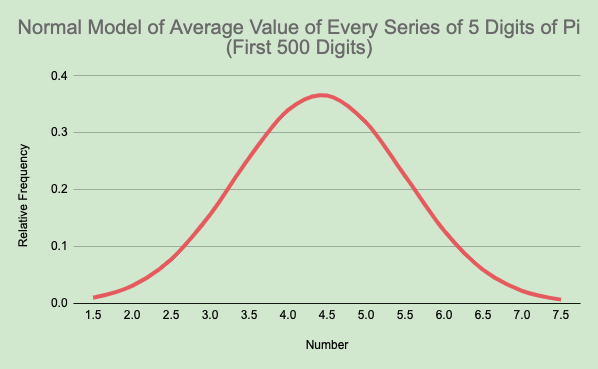
\includegraphics[width=\textwidth]{normdist.png}}
 
\section{Comparison of Distribution to Normal Model}
{69\% (69/100) of our data are within 1 standard deviation of the mean.}
{95\% (95/100) of our data are within 2 standard deviations of the mean.}
{100\% (100/100) of our data are within 3 standard deviations of the mean.}
{These percentages are approximately equal to 68\%, 95\%, and 99.7\%. The original distribution has an approximately symmetrical distribution just like the Normal Model. Thus, the Normal Model is useful because the original distribution is similar to the Normal Model which allows us to make conclusions from the original data based off the Normal Model.}
 
\bibliographystyle{unsrt}  
 
\begin{thebibliography}{1}
 
{“Digits of Pi - Up to 1 Million Digits.” Digits of Pi - Up to 1 Million Digits, Angio Dot Net, 3 Jan. 2016, 5:59:22, www.angio.net/pi/digits.html.}
 
\end{thebibliography}
 
\end{document}